\documentclass[class=book, crop=false,12 pt]{standalone}
\usepackage[subpreambles=true]{standalone}
\usepackage{import}
\RequirePackage{/home/mark/Documents/gradschool/research/thesis/preamble}

\begin{document}

\chapter{Conditions for Infinite Generation}
\label{ch:general}

Throughout this chapter $(G,(U_\alpha)_{\alpha\in \Phi},T)$ will be an RGD system of type $(W,S)$ and associated twin building $\Delta$ with the following assumptions:
\smallskip
\begin{equation}
	\label{assume}
	\tag{A} 
\begin{aligned}
	&S=\{s,t,u\},\: a=m(s,t),b=m(s,u),c=m(t,u)\\
	&3\le a,b,c<\infty\\
	&U_\alpha \text{ is finitely generated for all }\alpha\in \Phi\\
	&[U_\alpha,U_\beta]=1\text{ when }\alpha,\beta \text{ are nested}
\end{aligned}
\end{equation}

Before moving on we should address each one of these conditions to determine what role it will play. The first condition simply says that the twin building $\Delta$ is 2-dimensional. The second condition excludes the possibility of Moufang bigons as rank 2 links, and it ensures that every link will be strictly Moufang. If a root group $U_\alpha$ is not finitely generated, then it is easy to show that $U_+$ is also not fintiely generated, so we insist  $U_\alpha$ is finitely generated to be able to say anything interesting at all. In most of the known examples, the groups $U_\alpha$ are additive groups of vector spaces over some field. In these cases, reqiring the $U_\alpha$ to be finitely generated is equivalent to reqiring them to be finite. Finally, the condition that $[U_\alpha,U_\beta]=1$ if $\alpha,\beta$ are nested is a strengthening of the commutator relations in $G$ which will allow us to define certain homomorphisms in a nice way.

It is important to note that we are not being too restrictive, and there are still lots of examples of RGD systems which satisfy these properties. For example, we can construct Kac-Moody groups whose Weyl group will satisfy conditions (1) and (2). Furthermore, if the Kac-Moody group is over a finite field, then condition (3) will be satisfied, and conditions (1) and (2) will imply condition (4).

Throughout the remainder, we will see multiple diagrams showing models of the Coxeter complex of $W.$ To the reader familiar with hyperbolic geometry, these diagrams will appear to live in the Poincar\'{e} disk model of $\mathbb{H}^2.$ This is no accident, as conditions (1) and (2), along with the assumption that at least one of $a,b,c$ is at least 4, will imply that we can realized the Coxeter complex as a triangular tiling of the hyperbolic plane. The existence of a vertex with exceptional link will force $\max(a,b,c)\ge 4$ and thus the Coxeter complexes in question will satisfiy the necessary properties. Python code computing the hyperbolic geometry and generating the tikz diagrams can be found in Appendix \ref{ch:app}.

We know by Corollary \ref{cor:cofg} that $U_+$ is finitely generated if $\Delta$ has no exceptional rank 2 links. In the next two chapters we will determine when the same result will hold if $\Delta$ does have exceptional links. The general idea of the proof is as follows. For any vertex $v$ with an exceptional link we have a surjective homomorphism $\phi_v:U_v\to H$ where $H$ is cyclic and thus abelian. We will attempt to extend this homomorphism to all of $U_+$ in such a way that $U_\beta$ is sent to the identity if $U_\beta\not\subset U_v.$ Since $\phi_v$ is surjective, the extension will also be surjective, and therefore any generating set of $U_+$ must contain at least 1 element of $U_v.$ If we can do this for ``enough'' $U_v$ then we can potentially use this to prove that $U_+$ cannot be finitely generated. The difficulty lies in checking that the desired extension will be well defined, but we have a presentation of $U_+$ so it becomes a matter of checking that certain commutator relations are satisfied. Moreover, since the co-domain is abelian, commutators will automatically vanish which simplifies the conditions which need to be checked.

\section{Extension of $\phi_v$}
Let $\Sigma$ be the Coxeter complex of $W$ with fundamental chamber $C,$ and $\Phi_+$ be the positive roots of $\Sigma.$ We will also let $U_+=\langle U_\alpha|\alpha\in \Phi_+\rangle$ be the subgroup of $G$ generated by the positive root groups. The Moufang property implies that $a,b,c\in \{2,3,4,6,8\}$ and thus \eqref{assume} implies that $a,b,c\in \{3,4,6,8\}.$ We will also assume that $\Delta,$ and thus $\Sigma,$ has a vertex $v$ such that $\lk(v)$ is the building associated to one of the 4 exceptional Moufang polygons. Without loss of generality we will say that $v$ has type $s,$ and thus $c=m(t,u)\ge 4.$

Let $v$ be a vertex of $\Sigma$ such that $\lk(v)$ is the Moufang polygon associated to $C_2(2),G_2(2),G_2(3),$ or ${}^2F_4(2).$ Equivalently, this means $[U_v:U'_v]\ge 2.$ As described in the previous chapter we will let $\alpha_1,\dots,\alpha_n$ be a standard ordering of the positive roots through $v$ and we will define $U_i=U_{\alpha_i}$ for all $1\le i\le n.$ By Corollary \ref{cor:phiv}, there is a surjective homomorphism $\phi_v:U_v\to H$ where $H$ is a cyclic group and $\phi_v(U_1)=\phi_v(U_n)=\{1\}.$ We would like to extend $\phi_v$ to a map $\tilde{\phi}_v:U_v\to H$ in a specific way to use later. Our first lemma will define our notion of extending $\phi_v,$ and give a sufficient condition for this extension to exist.

\begin{lemma}
	\label{lem:existence}
	Suppose that $v$ is a vertex of $\Sigma$ such that $U'_v=\langle U_1,U_n\rangle\neq U_v,$ where $U_1,U_n$ are the simple root groups at $v.$ Then there is a surjective group homomorphism $\phi_v:U_v\to H$ with the property that $\phi_v(U_1)=\phi_v(U_n)=\{1\},$ where $H$ is a cyclic group. Also suppose that for any positive root $\gamma$ with $v\in \partial \gamma$ which is not simple at $v,$ that $\gamma$ is simple at $y$ for all $y\in \partial \gamma$ with $y\neq v.$ Then the map $\tilde{\phi}_v:\cup_{\gamma\in \Phi_+}U_\gamma\to H$ defined by
\[
	\tilde{\phi}_v(u)=\begin{cases} \phi_v(u)&\text{if }u\in U_\gamma\text{ and }v\text{ lies on }\partial\gamma\\
		1&\text{ otherwise}
	\end{cases}
\]
extends uniquely to a well defined group homomorphism $\tilde{\phi}_v:U_+\to H.$
\end{lemma}
\begin{proof}
	Since $U'_v\neq U_v$ we know that the map $\phi_v$ exists by Corollary \ref{cor:phiv}. We have a presentation for $U_+$ and we have defined $\tilde{\phi}_v$ on the generators of $U_+,$ so in order to check that it is well defined we will need to verify that the relations of $U_+$ are satisfied in the image.

	There are three types of relations in the presentation for $U_+.$ There are relations within the same root group $U_\alpha$ for all positive roots $\alpha.$ There are also relations between root groups of pre-nilpotent pairs where either the walls intersect or the roots are nested.

	Let $R_\alpha$ be a relation for $U_\alpha$ where $R_\alpha$ is considered as a word with letters in $U_\alpha.$ If $v$ lies on $\partial \alpha$ then $\tilde{\phi_v}(R_\alpha)=\phi_v(R_\alpha)=1$ since $\phi_v$ is a well defined homomorphism. Otherwise, every element of $U_\alpha$ is sent to 1 and thus $\tilde{\phi_v}(R_\alpha)=1$ as well so that $R_\alpha$ is mapped to the identity as desired.

	Now suppose that $\alpha$ and $\beta$ are any two positive roots. If $\alpha,\beta$ nested, then \eqref{assume} tells us that $[U_\alpha,U_\beta]=1.$ Since the co-domain of $\tilde{\phi_v}$ is an abelian group, then any relation of the form $[x,y]=1$ will be satisfied by the image.


	Now suppose that $\partial \alpha$ and $\partial \beta$ meet at a point $y$ and consider any relation of the form $[u_\alpha,u_\beta]=w$ where $u_\alpha\in U_\alpha,$ $u_\beta\in U_\beta,$ and $w$ is a word in $U_{(\alpha,\beta)}\subset U_y.$ Again, note that the image of the left side of this equation will always be the identity as the co-domain is still abelian. If $y=v$ then $U_y=U_v$ and thus $\tilde{\phi_v}(w)=\phi_v(w)=1$ because $\phi_v$ is well defined.

	Now suppose that $y\neq v.$ Then we can label the positive roots passing through $y$ as $\gamma_1,\cdots,\gamma_r$ in such a way that $(\gamma_i,\gamma_j)=\{\gamma_{r}|i<r<j\}$ whenever $i<j.$ In this case we can can say without loss of generality that $\alpha=\gamma_l$ and $\beta=\gamma_m$ with $l<m.$  There can be at most one root whose wall passes through $y$ and $v,$ which we will call $\gamma_k$ if it exists. If $\gamma_k$ does not exist, or $k\le l$ or $k\ge m$ then the root $\gamma_k$ is not contained in $(\alpha,\beta)$ and thus $\tilde{\phi_v}(U_\delta)=1$ for all $\delta\in (\alpha,\beta).$ This means $\tilde{\phi_v}(w)=1$ and the relation is satisfied.

	Now we suppose that $\gamma_k$ exists and $l<k<m.$ Then $\gamma_k$ is not simple at $y$ and thus $\gamma_k$ must be simple at $v$ by assumption. This means $\tilde{\phi_v}(U_{\gamma_k})=\phi_v(U_{\gamma_k})=1$ by the construction of $\phi_v.$ Since $\tilde{\phi_v}(U_{\gamma_i})=1$ for all $i\neq k$ by definition, this means that $\tilde{\phi_v}(w)=1$ showing the relation is satisfied and giving the desired result.
\end{proof}

Now Lemma \ref{lem:existence} gives a sufficient condition for the existence of $\tilde{\phi_v}$ which is fairly easy to check. This will be the main tool we use in the remainder of the section. 

Recall from our assumption \eqref{assume} that $(W,S)$ is a rank 3 Coxeter system with $S=\{s,t,u\},$ and $m(s,t)=a,m(s,u)=b,m(t,u)=c.$ We assumed that $3\le a,b,c.$ Let $C$ be the fundamental chamber of $\Sigma$ and let $x$ be the vertex of $C$ of type $s,$ so that $|\st(v)|=2c.$ If we assume that $\Sigma$ does contain exceptional links then we can say without loss of generality that $[U_x:U'_x]\ge 2$ so that $\phi_x$ exists. We would like to apply Lemma \ref{lem:existence} to show that $\tilde{\phi}_x$ exists, but before we do so we need the following result.

\begin{lemma}
\label{lem:xpos}
	Let $x$ be the vertex of $C$ of type $s.$ If $\gamma$ is any positive root at $x,$ and $y$ is any other vertex on $\partial\gamma,$ then $\gamma$ is simple at $y.$
\end{lemma}
\begin{proof} 
	Suppose that $\gamma$ is not simple at $y.$ Then we can label the positive roots at $y$ as $\delta_1,\dots,\delta_m$ in such a way that $\delta_i\cap \delta_j\subset \delta_k$ for $1\le i\le k\le j.$ In this case we have $\delta_1,\delta_m$ are simple at $y$ and $\gamma=\delta_r$ for some $1<r<m.$ But $x$ is a vertex of $C$ and $C\in \delta_1\cap \delta_m$ and thus $x\in \delta_1\cap \delta_m$ as well. We know that $x$ lies on $\partial \delta_r$ by assumption and thus $x$ is an element of $\partial \delta_r \cap \delta_1\cap \delta_m.$ But this is impossible as we can observe from the geometry of $\Sigma$ that $\partial \delta_i\cap \delta_1\cap \delta_m=\{y\}$ for all $1<i<m.$ Thus $\gamma$ is simple at $y$ as desired.
\end{proof}
Despite some of the technical details the previous result should be intuitively clear. The walls through $y$ will divide $\Sigma$ into $2m$ regions, and the region which contains $C$ will be bounded by the two simple roots. Since $x$ lies on $\partial \gamma,$ it is impossible for any other roots through $y$ to be any ``closer'' to $C$ and thus $\gamma$ must be simple at $y$ as we proved.
\begin{cor}
	\label{cor:phix}
	Let $x$ be the vertex of $C$ of type $s,$ and assume that $[U_x:U'_x]\ge 2.$ Then the map $\tilde{\phi}_x$ as defined in Lemma $\ref{lem:existence}$ is well defined.
\end{cor}
\begin{proof}
	Let $\gamma$ be any non-simple, positive root through $x$ and let $y$ be another vertex on $\partial \gamma.$ Then by the previous lemma, $\gamma$ is simple at $y$ and thus $\tilde{\phi_x}$ exists by Lemma \ref{lem:existence}.
\end{proof}

The remainder of the section will be used to show that we can use $\tilde{\phi}_x$ and the $W$ action on $\Sigma$ to construct a large family of vertices $\{v\}$ for which $\tilde{\phi}_v$ exists.

Let $\alpha_1,\dots,\alpha_n$ be a standard ordering of the positive roots through $x.$ Recall from chapter 1 that we can describe any root in terms of a pair of adjacent chambers. We can also identify $\mathcal{C}(\Sigma)$ with $W$ where the chamber $wC$ is associated to $w.$ If we use this identification then we can describe the roots as follows
\begin{align*}
	\alpha_1&=\{D\in \Sigma|d(D,C)<d(D,tC)\}=\{w\in W|\ell(w)<\ell(tw)\}\\
	\alpha_n&=\{D\in \Sigma|d(D,C)<d(D,uC)\}=\{w\in W|\ell(w)<\ell(uw)\}
\end{align*}
In a similar way we can define two more roots
\begin{align*}
	\beta&=\{D\in \Sigma|d(D,tC)<d(D,tsC)\}=\{w\in W|\ell(tw)<\ell(stw)\}\\
	\beta'&=\{D\in \Sigma|d(D,uC)<d(D,usC)\}=\{w\in W|\ell(uw)<\ell(suw)\}
\end{align*}
\begin{figure}[h]
	\label{fig:defineD}
	\begin{center}
	\resizebox{3.5in}{!}{\subimport{diagrams/}{defineD.tex}}
	\caption{The Roots $\alpha_1,\alpha_n,\beta,\beta'$ with the region $\D$ in yellow.}
\end{center}
\end{figure}

Now we can define $\mathcal{D}=\alpha_1\cap \alpha_n \cap \beta\cap \beta'.$ These roots are chosen and $\D$ is defined in such a way to give the following lemma:

\begin{lemma}
	\label{lem:containD}
	Let $x$ be the vertex of $C$ of type $s$ and assume $W=\langle s,t,u|s^2=t^2=u^2=(st)^a=(su)^b=(tu)^c=1\rangle.$ Let $\D=\alpha_1\cap \alpha_n\cap \beta\cap \beta'$ where $\alpha_1,\alpha_n,\beta,\beta'$ are roots of $\Sigma$ defined by
\begin{align*}
	\alpha_1&=\{D\in \Sigma|d(D,C)<d(D,tC)\}=\{w\in W|\ell(w)<\ell(tw)\}\\
	\alpha_n&=\{D\in \Sigma|d(D,C)<d(D,uC)\}=\{w\in W|\ell(w)<\ell(uw)\}\\
	\beta&=\{D\in \Sigma|d(D,tC)<d(D,tsC)\}=\{w\in W|\ell(tw)<\ell(stw)\}\\
	\beta'&=\{D\in \Sigma|d(D,uC)<d(D,usC)\}=\{w\in W|\ell(uw)<\ell(suw)\}
\end{align*}
If $\gamma$ is a positive root at $x$ which is not simple at $x,$ and $\delta$ is any other positive root such that $\partial\gamma\cap \partial\delta\neq \emptyset,$ then $\D\subset \gamma\cap \delta.$
\end{lemma}
\begin{proof}
	By assumption, $\gamma$ is a positive root through $x$ so $\gamma=\alpha_i$ for some $i.$ Furthermore, we assumed that $\gamma$ was not simple which means $2\le i \le n-1.$ Since $\alpha_1$ and $\alpha_n$ are simple at $x$ we can see that $\mathcal{D}\subset \alpha_1\cap \alpha_n\subset \alpha_i=\gamma.$ Thus it will suffice to prove that $\mathcal{D}\subset \delta.$

	Let $y=\partial\gamma \cap \partial \delta.$ If $y=x$ then $\delta$ is also a root which passes through $x$ and so $\delta=\alpha_j$ for some $j\neq i.$ Then as before we get $\alpha_1\cap \alpha_n\subset \alpha_j=\delta$ and thus $\mathcal{D}\subset \delta$ so that $\mathcal{D}\subset \gamma\cap \delta$ as desired.

	Now suppose that $\partial \gamma\cap \partial \delta=y\neq x.$ From the local geometry of $\Sigma$ around $x$ we can see the following facts. For any $\alpha_i$ with $2\le i\le n-1$ we know that $\partial\alpha_i\cap \alpha_1\cap \alpha_n=\{x\}$ and $\partial\alpha_i\subset \alpha_1\cup\alpha_n.$ Thus the point $y$ will lie in exactly one of $\alpha_1$ or $\alpha_n.$

	First suppose that $y\in \alpha_n$ so that $y\not\in \alpha_1.$ If $\partial\alpha_1\cap \partial\delta=\emptyset$ then there are exactly 4 possibilities. Either $\alpha_1\subset \delta,$ $\delta\subset\alpha_1,-\delta\subset \alpha_1,$ or $\alpha_1\subset -\delta.$ The last case is impossible as $C$ is a chamber of $\alpha_1$ but it is not a chamber of $-\delta.$ The cases $\delta\subset \alpha_1$ and $-\delta \subset \alpha_1$ are also impossible as they would contradict our assumption that $y\not\in \alpha_1$ and thus we get $\alpha_1\subset \delta$ and thus $\D\subset \alpha_1\subset \gamma\cap\delta$ as desired.

	Alternatively, assume that $\partial\alpha_1\cap \partial\delta=y'.$ Then the points $x,y,y'$ will form a triangle with sides on walls of $\Sigma.$ Then by the triangle condition, these three vertices must form a chamber, call it $E.$ The points $x,y$ lie on $\partial\gamma=\partial\alpha_i$ and the points $x,y'$ lie on $\partial\alpha_1.$ Since $y$ and $y'$ are adjacent this means that either $\gamma=\alpha_2$ or $\gamma=\alpha_n.$ The latter is a contradiction of our assumptions and thus $\gamma=\alpha_2.$ We know that $y$ and $y'$ are adjacent and $y\in \alpha_n.$ Since neither $y$ or $y'$ lies on $\partial\alpha_n$ this means that $y'\in \alpha_n$ as well.

	\begin{figure}[h]
%\resizebox{6.5 in}{!}{\subimport{diagrams/}{containD.tex}}
	\begin{center}
	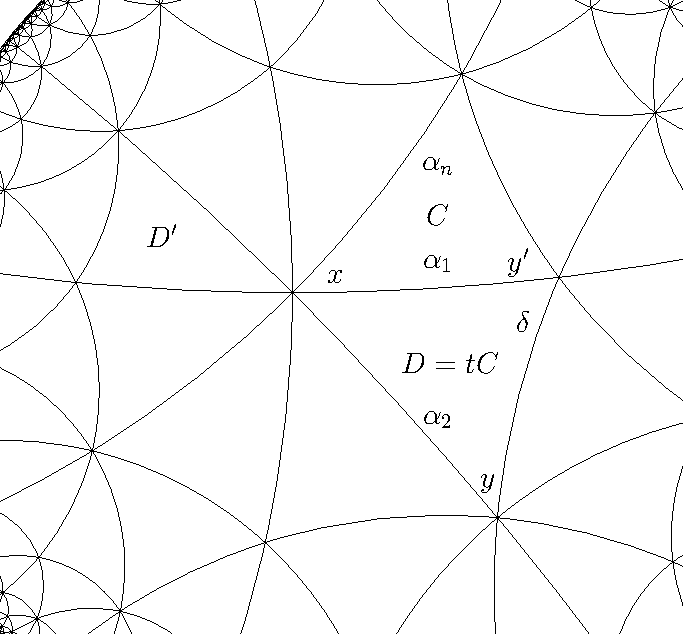
\includegraphics[width=3.5 in]{diagrams/containD.pdf}
\end{center}
\caption{$\partial\alpha_1\cap \partial\delta=y'$}
	\label{fig:localpic}
\end{figure}

	We know that $E$ is a chamber in $\st(x)$ with a side on $\partial \alpha_1$ and $\partial\alpha_2.$ Let $D=tC$ and $D'$ be the chamber opposite $D$ in $\st(x).$ Then either $E=D$ or $E=D'.$ By definition, $\partial\alpha_1$ is the only wall separating $C$ and $tC$ which means $D=tC\in \alpha_n.$ If $E=D'$ then $D'\in \alpha_n$ since $x,y,y'$ all lie in $\alpha_n.$ But this is a contradiction as $\alpha_n$ cannot contain two opposite chambers in $\st(x).$ Thus $E=D=tC$ and $\delta=\beta$ by definition. Thus $\D\subset \beta=\delta$ and $\D\subset \gamma\cap \delta$ as desired. A depiction of this situation can be found in Figure \ref{fig:localpic}.

	If we assume instead that $y\in\alpha_1$ so that $y\not\in \alpha_n$ then identical arguments show that $\delta=\beta'$ and we can again conclude that $\D\subset \gamma\cap \delta$ as desired.

%Now suppose $y\neq x$ and also assume that $x$ and $y$ are not adjacent. Suppose that $\partial \delta$ meets $\partial \alpha_1$ at a point $y'.$ Then the points $x,y,y'$ form a triangle, whose sides lie on the walls $\partial \gamma,$ $\partial \delta,$ and $\partial \alpha_1.$ The triangle condition then implies that $xyy'$ must be a chamber of $\Sigma,$ which is a contradiction since $x$ and $y$ are not adjacent. Thus $\partial \delta$ does not meet $\partial \alpha_1$ and a similar argument shows that $\partial \delta$ does not meet $\alpha_n.$ 
%
%From the geometry of the Coxeter complex, we can observe that for any $1<i<n$ we have $\partial \alpha_i \cap \alpha_1\cap \alpha_n=x.$ Since $y\neq x$ this means that $y$ does not lie in $\alpha_1\cap \alpha_n.$ We can assume without loss of generality that $y$ does not lie in $\alpha_1.$ We know that $\alpha_1$ and $\delta$ are two positive roots whose walls do not meet, and thus there are exactly three possibilites. Either $\alpha_1\subset \delta,$ $\delta\subset\alpha_1$ or $-\delta\subset \alpha_1.$ The later two cases are impossible as both would imply that $y\in \alpha_1$ which contradicts our assumption. Thus we have $\alpha_1\subset\delta$ which gives $\mathcal{D}\subset\alpha_1\subset \delta$ as desired.
%
%Now we suppose again that $y\neq x$ but $x$ and $y$ are adjacent. Then once again there are two possibilities. If $\partial \delta$ does not meet $\partial \alpha_1$ or $\partial \alpha_n$ then the identical argument from the last paragraph shows that $\mathcal{D}\subset \delta.$
%
%So now we suppose that $\partial \delta$ does meet $\partial \alpha_1$ or $\partial \alpha_n.$ If $\partial \delta$ meets $\partial \alpha_1$ at a point $y',$ then the vertices $xyy'$ will form a triangle which must be a chamber call it $C'.$ This chamber contains, $x,$ and has 2 sides on $\partial \alpha_1$ and $\partial \gamma$ respectively. Since $\gamma$ is not simple, an observation of the chambers around $x$ in Figure \ref{fig:defineD} shows that $\gamma$ must be $\alpha_2$ $C'$ must be $tC$ in which case $\delta=\beta$ by definition. Thus we get $\mathcal{D}\subset \beta =\gamma$ which proves the result.
%
%If $\partial \delta$ meets $\alpha_n$ then an identical argument shows that $\gamma=\beta'$ which also proves the result.
%
\end{proof}


We are now ready to construct a large family of vertices $\{v\}$ for which $\tilde{\phi_v}$ will exist. The idea is as follows. If we take any chamber in $\mathcal{D}$ and treat it as a new ``$C$'' then $\tilde{\phi_x}$ would exist for this ``$C.$'' So what we do is apply elements of $W$ which map the chambers of $\mathcal{D}$ to $C,$ and use these choices of $w$ to get new vertices $v.$ We can use Lemma \ref{lem:resporder} to show that this $W$ action will play nicely with the map $\phi_v.$

%Since the construction of these $\tilde{\phi_v}$ depends on properties of simple roots, we want to know the simplicity behaves nicely with the action of $W.$ To this end we have the following lemma.
%
%\begin{lemma}
%	Suppose $v$ is a vertex of $\Sigma$ with simple roots $\gamma,\gamma'$ at $v.$ If $w$ is an element of $w$ such that $w\delta$ is a positive root for all positive $\delta$ at $v,$ then $w\gamma$ and $w\gamma'$ are the simple roots at $wv.$ \label{preservesimple}
%	\Huge I don't know if I need this any more, check the lemma from Chapter \ref{ch:known} \normalsize
%\end{lemma}
%\begin{proof}
%	Let $\delta$ be a positive root at $wv.$ Since $w$ induces an isomorphism of simplical complexes, and it sends positive roots at $v$ to positive roots at $wv,$ it must also send negative roots at $v$ to negative roots at $wv.$ So $w^{-1}\delta$ is a root at $v,$ and $w(w^{-1}\delta)=\delta$ is positive, so $w^{-1}\delta$ is also positive. Thus by definition of simple, we have $\gamma \cap \gamma'\subset w^{-1}\delta.$ But we can now apply $w$ to get $w\gamma \cap w\gamma' \subset \delta.$ Since the choice of $\delta$ was arbitrary we must have $w\gamma$ and $w\gamma'$ are simple as desired.
%\end{proof}

\begin{lemma}
	\label{lem:Dexists}
	Let $x$ be the vertex of $C$ of type $s,$ and assume $U'_x\neq U_x.$ If $v$ is a vertex in $\mathcal{D}=\alpha_1\cap \alpha_n\cap \beta \cap \beta'$ of type $s$ then there is a $w\in W$ such that $w^{-1}x=v$ and $\tilde{\phi}_{wx}$ exists.
\end{lemma}
\begin{proof}
	Let $D=\mathrm{Proj}_{v}(C)$ and define $w$ so that $D=w^{-1}C.$ By definition, $v$ is a vertex of $D$ of type $s$ and $w^{-1}x$ is also a vertex of $D$ of type $s$ and thus $w^{-1}x=v.$ The claim is that this $w$ will satisfy the desired properties. First we mention that $wx$ is also a vertex of $\Sigma$ of type $s$ and thus $[U_{wx}:U'_{wx}]\ge 2$ and $\phi_{wx}$ exists by Corollary \ref{cor:respectphiv}. 
	
	Again, the definition of projections means that $D$ is the closest chamber to $C$ which has a vertex of $w^{-1}x.$ Since $\mathcal{D}$ is convex, and $w^{-1}x$ and $C$ both lie in $\mathcal{D},$ we also know that $D=\mathrm{Proj}_{w^{-1}x}(C)$ lies in $\mathcal{D}$ as well. By a similar argument we know that $\mathrm{Proj}_{x}(D)$ must lie in $\mathcal{D}\subset \alpha_1\cap \alpha_n$ and thus $\mathrm{Proj}_{x}(D)=C.$ Now define $E=wC$ and note that the action of $W$ respects projections and thus we have
	\[
		E=wC=\mathrm{Proj}_{wx}{wD}=\mathrm{Proj}_{wx}{C} \qquad C=wD=\mathrm{Proj}_{w(w^{-1}x)}{wC}=\mathrm{Proj}_{x}{E}
	\]
In particular, a root through $wx$ is positive if and only if it contains $E.$

Our goal is to apply Lemma \ref{lem:existence} at the vertex $wx.$ Now suppose that $\gamma$ is a non-simple, positive root through $wx$ and $y$ is another vertex on $\partial \gamma.$ We must show that $\gamma$ is simple at $y.$ Since $\gamma$ is positive through $wx$ we know that $C,E\in \gamma.$ If we apply $w^{-1}$ then we get the following facts. We know that $w^{-1}\gamma$ is a root such that $\partial (w^{-1}\gamma)$ passes through $w^{-1}wx=x.$ We also know that $w^{-1}C=D,w^{-1}E=C\in w^{-1}\gamma$ so that $w^{-1}\gamma$ is also a positive root. Since $w^{-1}$ sends positive roots at $wx$ to positive roots at $x$ we can apply Lemma \ref{lem:resporder} when necessary.

The first claim is that $w^{-1}\gamma$ is not simple at $x.$ Suppose that $\delta$ is any positive root at $wx.$ Then $E\subset \delta$ and so applying $w^{-1}$ we get that $w^{-1}E=C\subset w^{-1}\delta.$  By Lemma \ref{lem:resporder} this means that $w^{-1}$ sends simple roots at $wx$ to simple roots at $x.$ Since $\gamma$ is not simple at $wx$ this means that $w^{-1}\gamma$ is not simple at $x.$

So $w^{-1}\gamma$ is a non-simple positive root at $x,$ and since $y$ lies on $\partial \gamma$ we also know that $w^{-1}y$ lies on $w^{-1}(\partial \gamma).$ If we apply Lemma \ref{lem:xpos} we can see that $w^{-1}\gamma$ must be simple at $w^{-1}y.$ 
\begin{figure}[h]
	\label{fig:mappicture}
\resizebox{6.5 in}{!}{\subimport{diagrams/}{mappicture.tex}}
\caption{The effect of $w$ and $w^{-1}$ on the chambers and roots.}
\end{figure}


Recall that $D\in \mathcal{D}$ by assumption. Now suppose that $\delta$ is any positive root at $w^{-1}y.$ Then by Lemma \ref{lem:containD} we know that $D\in \mathcal{D}\subset \delta.$ If we apply $w$ then we get $C=wD\in w\delta$ and $w\delta$ is a root through $y.$ Thus $w\delta$ is a positive root through $y$ and therefore $w$ sends positive roots through $w^{-1}y$ to positive roots through $y.$ Again we can apply Lemma \ref{lem:resporder} to say that $w$ must also send simple roots through $w^{-1}y$ to simple roots through $y.$ But $w^{-1}\gamma$ was a simple root through $w^{-1}y$ and thus $\gamma$ is simple at $y$ as desired.

We now have a vertex $wx$ where $[U_{wx}:U'_{wx}]=[U_x:U'_x]\ge 2$ and the positive roots at $wx$ which are not simple at $wx$ are simple everywhere else. Thus we can apply Lemma \ref{lem:existence} to say that $\tilde{\phi}_{wx}$ exists as desired.
\end{proof}

Now we have shown that vertices of $\D$ in some way correspond to $\tilde{\phi_v}.$ If our goal is to find infinitely many such $v$ then there is still some work to be done. For instance, we do not yet know if the region $\D$ contains infinitely many chambers, or even if it does, if all the vertices of $D$ lie on finitely many walls. We will show in the next section that these issues are not a problem in most cases.


\section{When $\D$ is infinite}
Our first task will be two show that the region $\D$ contains infinitely many vertices. Intuitively, this will happen if the walls for $\beta$ and $\beta'$ do not meet, and we will first give a sufficient (and necessary) condition for this.

Recall that $W$ is defined by the edge labels $a=m(s,t),b=m(s,u),c=m(t,u)$ we assumed that the vertices of type $s$ were exceptional which implies $c\ge 4.$ We will show that if we also assume that $b\ge 4$ then the region $\mathcal{D}$ will contain infinitely many chambers.


\begin{lemma}
	\label{lem:infmany}
	Let $(W,S)$ be a rank 3 Coxeter system defined by $a=m(s,t),b=m(s,u),c=m(t,u)$ with $3\le a$ and $4\le b,c.$ If we let $w_k=(tus)^k$ for all $k\ge 0,$ then the vertices $(w_k)^{-1}x$ are all distinct from one another and all lie in $\mathcal{D}.$
\end{lemma}
\begin{proof}
	Note that $(w_k)^{-1}=(sut)^k$ for all $k.$ First we will show that $(w_k)^{-1}x\in \D$ for all $k.$ Since $x$ is a vertex of $C$ we know that $(w_k)^{-1}x$ is a vertex of $(w_k)^{-1}C$ and thus it will suffice to show $(w_k)^{-1}C$ is contained in $\D$ for all $k.$ Since the roots $\alpha_1,\alpha_n,\beta,\beta'$ can be identified with their corresponding subsets of $W,$ we can use the length function to check containment in these roots.

Now we recall the two $M$ operations on words in a Coxeter group are as follows:
\begin{enumerate}
	\item Delete a sub-word $ss$ for some $s\in S$
	\item Replace a sub-word of the form $stst\cdots st(s)$ by a sub-word of the form $tsts\cdots ts(t)$ where each of these strings has length $m(s,t).$
\end{enumerate}
Also recall that any word in a Coxeter group can be reduced to its minimum length by repeated application of these operations, and any two reduced words can be converted each other by application of operations of type 2. Therefore, in order to check that the length relations are satisfied, it will be enough to show that we can never perform an $M$ operation of type 1 as this is the only way to reduce length.

It is immediate from the definition that $\ell((w_k)^{-1})=3k$ for all $k.$ We can also see that $\ell(t(w_k)^{-1})=3k+1$ and thus $(w_k)^{-1}\in \alpha_1$ for all $k.$ Similarly, $u(w_k)^{-1}=u(sutsut\cdots),$ and no reduction operations can be done as we assumed $m(s,u)\ge 4.$ Thus $\ell(u(w_k)^{-1})=3k+1$ which means $(w_k)^{-1}\in \alpha_n$ as well.

	Now consider the element $st(w_k)^{-1}.$ If we write this element out in terms of the generators and apply the only possible Coxeter relations we get
	\begin{align*}
		st(w_k)^{-1}&=st(sutsut\cdots)\\
		     &=(sts)(utsuts\cdots)\\
		     &=(tst)(utsuts\cdots)\\
		     &=(ts)(tut)(sutsut\cdots)
	\end{align*}
	and none of these can be reduced as $m(t,u)\ge 4.$ Note that the commutation relation $sts=tst$ may not be possible if $m(s,t)\ge 4,$ but it is the only relation possible in $st(w_k)^{-1}$ and even if it does exists then it does not allow $st(w_k)^{-1}$ to be reduced in length. We previously showed $\ell(t(w_k)^{-1})=3k+1$ and now we see $\ell(st(w_k)^{-1})=3k+2$ and so $(w_k)^{-1}\in \beta.$

	Now we can consider $su(w_k)^{-1}$ in a similar manner. Writing $su(w_k)^{-1}$ out as a word in the generators and applying Coxeter relations gives us
\begin{align*}
	su(w_k)^{-1}&=su(sutsut\cdots)\\
	     &=(susu)(tsutsu\cdots)\\
	     &=(usus)(tsutsu\cdots)\\
	     &=(usu)(sts)(utsuts\cdots)\\
	     &=(usu)(tst)(utsuts\cdots)
\end{align*}
Note once again that not all of these relations may be possible if $m(s,u)=6$ or $m(s,t)\ge 4.$ However, these are the only possible relations, and since $su(w_k)^{-1}$ cannot be reduced under these assumptions, it cannot be reduced at all. Thus $\ell(su(w_k)^{-1})=3k+2$ which means $su(w_k)^{-1}\in \beta'$ as well.

Now it only remains to show that $v_m\neq v_n$ for $m\neq n.$ Suppose $(w_m)^{-1}x=(w_n)^{-1}x$ for $m>n.$ Then we would have $x=w_m(w_n)^{-1}x=w_{m-n}.$ Thus it will suffice to show $w_kx\neq x$ for any $k\ge 1.$ But we know that $\mathrm{stab}_{W}(x)=\langle u,t \rangle$ which does not contain $w_k$ for any $k\ge 1$ and thus $(w_k)^{-1}x\neq x$ so that $(w_m)^{-1}x\neq (w_n)^{-1}x$ as desired.

\end{proof}

We now know that each of the $(w_k)^{-1}x$ is distinct and each of them lies in $\D.$ By Lemma \ref{lem:Dexists} we know that $\tilde{\phi}_{w_kx}$ exists for each $k\ge 0.$ Our idea is still to use each of these vertices to give a root which must be contained in any generating set. However, there is still one possible issue. If almost all of these vertices lie on the same wall, then an inclusion of that root in a generating set could satisfy infinitely many of the $k$ at once, which would not allow us to prove infinite generation. So it remains to show that not only are the vertices $w_nx$ distinct, but also no two lie on the same wall.

\begin{lemma}
	\label{lem:samewall}
	Let $w_k=(tus)^k$ for all $k\ge 0$ and $x$ the vertex of $C$ of type $s.$ If $W$ as in the rest of this section with $3\le a,4\le b,c$ then $w_mx$ and $w_nx$ do not lie on the same wall of $\Sigma$ if $m>n\ge 0.$
\end{lemma}
\begin{proof}
	Suppose $w_mx$ and $w_nx$ do lie on the same wall with $m>n.$ Then we also know that $w_nw^{-1}_mx=w_{n-m}x$ and $x$ will lie on the same wall. Since $m>n$ we can let $k=m-n$ and thus it will suffice to show that $(w_k)^{-1}x$ and $x$ do not lie on the same wall for any $k\ge 1.$
	
We know from Lemma \ref{lem:infmany} that $(w_k)^{-1}x\in \D.$ Thus if $(w_k^{-1})x$ and $x$ lie on the same wall, it must be a wall through $x$ and thus it must be $\partial\alpha_i$ for some $i.$ We know that $(w_k^{-1})x\in \alpha_1\cap \alpha_n$ since $\D\subset \alpha_1\cap \alpha_n$ by definition. But we can also recall that $\partial\alpha_j\cap \alpha_1\cap \alpha_n=\{x\}$ for $2\le j\le n-1.$ Thus we have $i=1$ or $i=n$ so that $(w_k^{-1})x$ either lies on $\partial\alpha_1$ or $\partial\alpha_n.$  Therefore, we either have $u(w_k)^{-1}x=(w_k)^{-1}x$ or $t(w_k)^{-1}x=(w_k)^{-1}x$ which implies that either $w_kuw_k^{-1}$ or $w_ktw_k^{-1}$ is contained in $\mathrm{stab}_W(x)=\langle u,t \rangle.$ However, by a similar argument as before, we can simply write out these elements and show that they cannot be reduced. The only possible relations we have are
\begin{align*}
	w_ktw_k^{-1}&=(\cdots tustus)t(sutsut\cdots)\\
		    &=(\cdots tustu)(sts)(utsut\cdots)\\
		    &=(\cdots tustu)(tst)(utsut\cdots)
\end{align*}
or
\begin{align*}
	w_kuw_k^{-1}&=(\cdots stustus)u(sutsuts\cdots)\\
		    &=(\cdots stust)(ususu)(tsuts\cdots)\\
		    &=(\cdots stust)(sus)(tsuts\cdots)\\
		    &=(\cdots stu)(sts)u(sts)(uts\cdots)\\
		    &=(\cdots stu)(tst)u(tst)(uts\cdots)\\
\end{align*}
since $m(t,u)\ge 4.$ Similarly as before, even these relations are only possible if $m(s,u)=4,$ but even in that case we cannot eliminate every instance of $s$ in $w_kuw_k^{-1}.$ In both cases we can see that there is no further reduction possible and thus neither of these conjugates can possibly lie in $\langle u,t \rangle.$ Thus the $w_nx$ all lie on distinct walls as desired.
\end{proof}

We now have all the ingredients and are ready to prove the main theorem.

\begin{theorem}
	\label{thm:notfg}
	Let $(G,(U_\alpha)_{\alpha\in \Phi},T)$ be an RGD system of type $(W,S)$ with associated building $\Delta$ which satisfies
	\begin{equation}
	\tag{A} 
\begin{aligned}
	&S=\{s,t,u\},\: a=m(s,t),b=m(s,u),c=m(t,u)\\
	&3\le a,b,c<\infty\\
	&U_\alpha \text{ is finitely generated for all }\alpha\in \Phi\\
	&[U_\alpha,U_\beta]=1\text{ when }\alpha,\beta \text{ are nested}
\end{aligned}
\end{equation}
Also assume that $x$ is the vertex of $C$ of type $s$ and that $\lk(x)$ is the building assoicated to one of the exceptional groups listed in Lemma \ref{lem:index}, implying $c\ge 4.$ If $b\ge 4,$ then the group $U_+=\langle U_\alpha|\alpha\in \Phi_+\rangle$ is not finitely generated.


\end{theorem}
\begin{proof}
	Suppose that $U_+$ is finitely generated. Then there is some finite set of roots $\beta_1,\dots,\beta_m$ such that $U_+=\langle U_{\beta_i}|1\le i\le m\rangle.$ Now no two of the vertices $(tus)^{-k}x$ lie on the same wall and thus we can choose $k$ so that $v=(tus)^{-k}x$ does not lie on $\partial \beta_i$ for any $i.$ By Lemma \ref{lem:infmany} and Lemma \ref{lem:Dexists} we know that $\tilde{\phi}_v$ exists, and by definition it is a surjective map from $U_+\to H$ where $H$ is a cyclic group. However, we can also see by the definition  of $\tilde{\phi}_v$ that $\tilde{\phi_v}(U_{\beta_i})=1$ for all $i,$ since none of these walls meet $v.$ But this means $\tilde{\phi_v}$ sends all of the generators of $U_+$ to the identity and thus it must be the trivial map which is a contradiction. Thus $U_+$ is not finitely generated as desired.
\end{proof}

In the previous proof we assumed that $b=m(s,u)$ and $c=m(t,u)$ are at least 4, but the labels are arbitrary and the previous theorem implies that $U_+$ is not finitely generated if there is an exceptional vertex, and any other vertex $v'$ has $|st(v')|\ge 8.$ The proof of Theorem \ref{thm:notfg} also implies a stronger statement.

\begin{cor}
	\label{cor:abnotfg}
	If $(G,(U_\alpha)_{\alpha\in \Phi},T)$ is an RGD system as defined in Theorem \ref{thm:notfg}, then $(U_+)_\text{ab}$ is not finitely generated.
\end{cor}
\begin{proof}
	Suppose that $(U_+)_\text{ab}$ is finitely generated. Then there is a finite set of roots $\beta_1,\dots,\beta_m$ such that the images $[U_{\beta_1}],\dots,[U_{\beta_m}]$ of the root groups generate $(U_+)_\text{ab}.$ As in the previous proof, we choose a vertex $v$ which does not lie on any $\partial \beta_i$ such that $\tilde{\phi}_v$ exists. We know $\tilde{\phi}_v(U_{\beta_i})=\{1\}$ for all $i.$ But the co-domain of $\tilde{\phi}_v$ is abelian, and thus the map will factor through $(U_+)_\text{ab}$ and we get a map $f:(U_+)_\text{ab}\to H$ where $f([u])=\tilde{\phi}_v(u).$ But then $f$ is also surjective, but $f([U_{\beta_i}])=\{1\}$ for all $i$ which is again a contradiction.
\end{proof}

In this chapter we were able to prove that $U_+$ will not be finitely generated when we have exceptional links and at least two labels which are at least 4. In the next chapter we will examine what happens in the remaining cases, meaning when two of our edge labels are 3.

\end{document}
